%***********************************************************************
% Lab Report Template
% R. W. Melton
% May 19, 2019
% August 24, 2020
%***********************************************************************
%Modify the following macros to set document property values
%used for cover sheet (title page) and page header
\newcommand{\CourseNumber}{CMPE-250}
\newcommand{\CourseName}{Assembly and Embedded Programming}
\newcommand{\SemesterName}{Fall 2020}
\newcommand{\SemesterCode}{20201}
\newcommand{\LabExNum}{9}
\newcommand{\LabExTitle}{Serial I/O driver}
\newcommand{\StudentName}{Andrei Tumbar}
\newcommand{\DateSubmit}{Submitted: 11-03-20}
\newcommand{\LabSection}{5}
\newcommand{\LabInstructor}{Gordon Werner}
\newcommand{\TAa}{Tianran Cui}
\newcommand{\TAb}{Anthony Bacchetta}
\newcommand{\LectureSection}{1}
\newcommand{\LectureInstructor}{Melton}
%End macros for document property values
%***********************************************************************
\title{Lab Ex. \LabExNum\ Report}
\author{\StudentName}
\date{\DateSubmit}
\makeatletter %make \title, \author, and \date availabile with \@
\newcommand{\FontSize}{12}
\newcommand{\FontUnit}{pt}
\newcommand{\HeadSize}{\dimexpr \FontSize\FontUnit + 2pt \relax}
\documentclass[\FontSize\FontUnit,letterpaper,oneside]{article}
\usepackage[twoside=false,margin=1in]{geometry}
\usepackage[utf8]{inputenc}
\usepackage[USenglish]{babel}
\usepackage{graphicx}
\usepackage[normalem]{ulem}
\usepackage{newtxtext, newtxmath}
%If newtx package had to be installed in multiuser environment
%regular user may have to run updmap command to avoid following error
%FATAL:  ``PK font ts1-qtmr could not be created.'' in miktex-makepk
%Alternatively, uncomment the following line
%\pdfmapfile{=pdftex35.map
\usepackage{booktabs}
\usepackage{enumitem}
\usepackage{nameref}
\usepackage{hhline}
\usepackage{fontspec,kantlipsum}
\usepackage[T1]{fontenc}
\usepackage{caption}
\captionsetup[table]{skip=10pt}
\usepackage[pdfborder={0 0 0},plainpages=false,pdfpagelabels]{hyperref}
\def\code#1{\texttt{#1}}
%If hyperref generates errors on first build, rebuild.            
\hypersetup{pdfauthor={\@author},
            pdftitle={\@title},
            pdfsubject={\CourseNumber\ \SemesterCode},
            %pdfkeywords={},
            %pdfproducer={Latex with hyperref, or other system},
            %pdfcreator={pdflatex, or other tool}
            urlcolor=none}
\setlength{\topsep}{\z@}
\setlength{\partopsep}{\z@}
\setlength{\itemsep}{\z@}
\setlength{\parindent}{\z@}
\setlength{\parskip}{\FontSize\FontUnit plus 2pt minus 1pt}
\setlength{\baselineskip}{\dimexpr \FontSize\FontUnit + 2pt \relax}
\renewcommand \baselinestretch{1}
\makeatletter
  \renewcommand \section{
    \@startsection{section}{1}{\z@}
      %Before 2 lines, accounting for normal \parskip
      {\dimexpr \FontSize\FontUnit * 2 - \parskip \relax plus 0pt minus 0pt}
      %After 1 line, accounting for normal \parskip
      {0.1pt plus 2pt minus 1pt} %nonzero amount to get normal \parskip
      {\normalfont\normalsize\bfseries}} 
  \renewcommand \subsection{
    \@startsection{paragraph}{2}{\z@}
      %Before 1 lines, accounting for normal \parskip
      {0.1pt plus 2pt minus 1pt}
      %After 0.5 em on same line as heading
      {-0.5em} 
      {\normalfont\normalsize\bfseries}} 
  \renewcommand \subsubsection{
    \@startsection{paragraph}{3}{\z@}
      %Before 1 line, accounting for normal \parskip
      {0.1pt plus 2pt minus 1pt}
      %After 0.5 em on same line as heading
      {-0.5em} 
      {\normalfont\normalsize\uline}} 
  \renewcommand \paragraph{
      \@startsection{paragraph}{4}{\z@}
      %Before 1 line, accounting for normal \parskip
      {0.1pt plus 2pt minus 1pt}
      %After 0.5 em on same line as heading
      {-0.5em} 
      {\normalfont\normalsize}} 
\makeatother
\pagenumbering{arabic}
\headheight=\HeadSize
\usepackage{fancyhdr}
\renewcommand{\headrulewidth}{0pt}
\renewcommand{\footrulewidth}{0pt}
\makeatletter %make \title, \author, and \date availabile with \@
\pagestyle{fancy}
\fancyhead{} %clear all header fields
\fancyhead[L]{\small \CourseNumber\ \SemesterCode \@author:  \@title}
\fancyhead[R]{\small Page \thepage\ of \pageref*{LastPage}}
\fancyfoot{} %clear all footer fields
\fancypagestyle{plain}{
  \renewcommand{\headrulewidth}{0pt}
  \renewcommand{\footrulewidth}{0pt}
  \fancyhf{} %clear header and footer fields
  \fancyfoot[C]{\small \CourseNumber\ \SemesterCode\ \@author:  \@title:  
    Page \thepage\ of \pageref*{LastPage}}
}
%May require second build to get correct page numbers.   


\usepackage{xcolor}
\usepackage{listings}

\definecolor{mGreen}{rgb}{0,0.6,0}
\definecolor{mGray}{rgb}{0.5,0.5,0.5}
\definecolor{mPurple}{rgb}{0.58,0,0.82}
\definecolor{backgroundColour}{rgb}{0.95,0.95,0.92}

\lstdefinestyle{CStyle}{
    commentstyle=\color{mGreen},
    keywordstyle=\color{magenta},
    numberstyle=\tiny\color{mGray},
    stringstyle=\color{mPurple},
    basicstyle=\footnotesize,
    breakatwhitespace=false,         
    breaklines=true,                 
    captionpos=b,                    
    keepspaces=true,                 
    numbers=left,                    
    numbersep=5pt,                  
    showspaces=false,                
    showstringspaces=false,
    showtabs=false,                  
    tabsize=2,
    language=C
}

         
\begin{document}
\raggedbottom
\widowpenalties 1 10000
\lefthyphenmin=4
\righthyphenmin=4
\setlist{nolistsep}
%***********************************************************************
%Title page is automatically generated from macros at top of file
\pagenumbering{roman}
\begin{titlepage}
  %No space before paragraph at top of page
  %\vspace{\dimexpr-2\parsep-2\parskip\relax}
  %1.5 in before center (list) at top of page
  \vspace*{\dimexpr 1.5in - \topsep - \partopsep - \topskip - \parskip \relax}
  \begin{center}
    \textbf{\large\CourseNumber\ \CourseName\linebreak
      \linebreak
      Laboratory Exercise \LabExNum\linebreak
      \linebreak
      \LabExTitle}
  \end{center}
  \vspace*{\dimexpr 1.5in - \topsep - \partopsep - \topskip \relax}
  \par By submitting this report, I attest that its contents are wholly 
    my individual writing about this exercise and that they reflect 
    the submitted code.  I further acknowledge that permitted 
    collaboration for this exercise consists only of discussions of 
    concepts with course staff and fellow students.  Other than code 
    provided by the instructor for this exercise, all code was 
    developed by me.
  \null
  \vspace*{4\parskip}
  \hspace*{3.25in}\begin{tabular}[t]
    {@{\hskip0pt}r    %Specification
     @{\hskip1em}l    %Value
     @{\hskip0pt}}
    \toprule[1pt]
    \multicolumn{2}{l}{\StudentName}\\
    \multicolumn{2}{l}{\DateSubmit}\\
    \\
    Lab Section:&\LabSection\\
    Instructor:&\LabInstructor\\
    TA:&\TAa\\
    &\TAb\\
    \\
    Lecture Section:&\LectureSection\\
    Lecture Instructor:&\LectureInstructor
  \end{tabular}
\end{titlepage}
\pagenumbering{arabic}
\thispagestyle{plain}
%***********************************************************************
%Report body begins here
After the program was written and compiled, the executable was loaded into a KL-05 board to be tested.

\begin{figure}[h!]
	\centering
	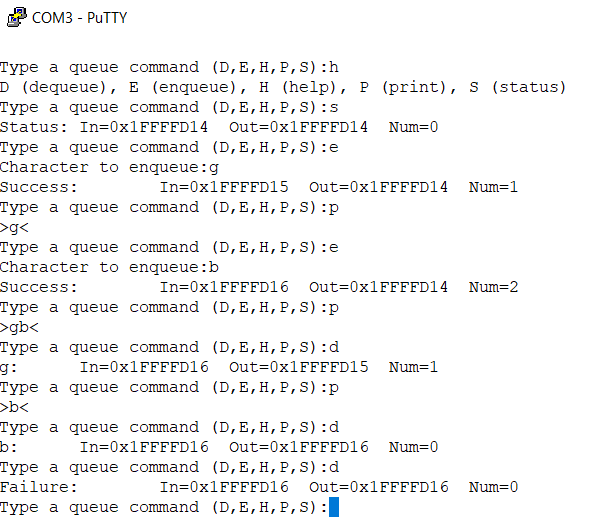
\includegraphics{capture}
	\caption{Terminal screen capture using interrupt for IO}
	\label{fig:capture1}
\end{figure}

Figure \ref{fig:capture1} shows the output of the terminal after each prompt command was used in various steps. The output is the same as from laboratory exercise 7. This is expected as the change being made in this exercise is the way the IO works not the way the main program works. Because the output is seen in both exercises, the 

\section*{Memory-map addresses}

\begin{table}[h!]
\begin{center}
\caption{Code section offsets and endings.}
\label{tab:q1}
\begin{tabular}{ |l||c|c| }
\hline
Subroutine & Start Address & Ending Address \\\hhline{|=||=|=|}
Executable code & \code{0x00000410} & \code{0x000008e3} \\\hline 
UART\_ISR & \code{0x0000075f} & \code{0x0000079c} \\\hline 
Constants & \code{0x000001c4} & \code{0x000002bb} \\\hline
Program Queue & \code{0x1ffffd00} & \code{0x1ffffd11} \\\hline
RxQueue & \code{0x1ffffd18} & \code{0x1ffffd29} \\\hline
TxQueue & \code{0x1ffffd2c} & \code{0x1ffffd3d} \\\hline
\end{tabular}
\end{center}
\end{table}

\label{LastPage}
\end{document}
